\section{Z-transformation}
\subsection{Z-transformation}
$$X(z)=\sum_{n=0}^{\infty}x(n)z^{-n}$$
Notation:
$$X(z)=\mathcal{Z}\{x(n)\}\qquad x(n)=\mathcal{Z}^{-1}\{X(z)\}$$
\subsubsection{s and z domain}
$$X_s(s)=X(z)\qquad \text{when }z=e^{st}\quad s=\displaystyle\frac{1}{T}\ln(z)$$
where $s=\sigma+j\omega$
\begin{center}
  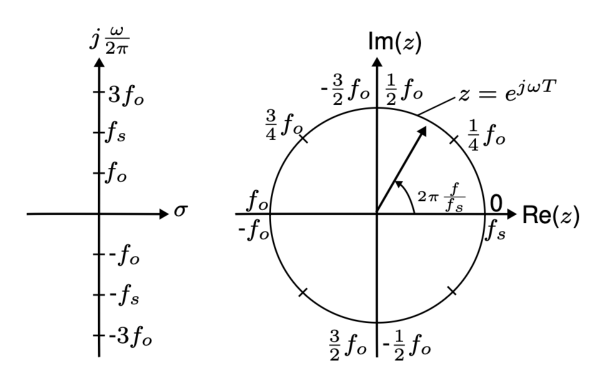
\includegraphics[width=0.5\textwidth]{Images/z-s_domain.png}
\end{center}
Here we see $\sigma<0$ is mapped inside the unit circle $|z|<1$.
\subsubsection{Transformation rules/pairs}

\begin{table}[h]
\centering
\begin{tabular}{|>{\columncolor[HTML]{C0C0C0}}c|c|c|}
\hline
\textbf{Rule}& $x(n)$& $X(z)$ \\ \hline
Z1& $ax_1(n)+bx_2(n)$&$aX_1(z)+bX_2(z)$\\ \hline
Z2& $x(n-m)$&$z^{-m}X(z)$ \\ \hline
Z3& $x(n)a^{-n}$ &$X(az)$ \\ \hline
Z4&$x(n)s^{-bn}$&$X(e^{bT}z)$ \\ \hline
Z5&$\sum_{m=0}^n x(m)h(n-m)$&$X(z)H(z)$ \\ \hline
\end{tabular}
\end{table}

\begin{table}[h]
\centering
\begin{tabular}{|>{\columncolor[HTML]{C0C0C0}}c|c|c|}
\hline
\textbf{Pair}& $x(n)$& $X(z)$ \\ \hline
ZT1& $\delta(n)$& $1$\\ \hline
ZT2& $u(n)$&$\frac{z}{z-1}$ \\ \hline
ZT3& $n$ &$\frac{z}{(z-1)^2}$ \\ \hline
ZT4&$a^n$&$\frac{z}{z-a}$ \\ \hline
ZT5&$e^{s_0nT}$&$\frac{z}{z-e^{s_0T}}$ \\ \hline
ZT6&$\sin(\omega_0nT)$&$\frac{\sin(\omega_0T)z}{z^2-2\cos(\omega_0T)z+1}$ \\ \hline
ZT7&$\cos(\omega_0nT)$&$\frac{z^2-\cos(\omega_0T)z}{z^2-2\cos(\omega_0T)z+1}$ \\ \hline
\end{tabular}
\end{table}

If $|x|<1$:
$$\sum_{i=0}^\infty=\frac{1}{1-x}$$

\subsection{Differential equations}
A N'th order differential equation, that describes a causal system:
$$y(n)+b_{1}y(n-1)+\cdots+b_{N}y(n-N)=a_{0}x(n)+a_{1}x(n-1)+\cdots+a_{N}x(n-N)$$
where $x(n-i)$ is the time-delayed input sequence, $y(n-i)$ is the time-delayed output sequence
and $a_i,b_i$ are real koefficients.

This can also be written as:
$$y(n)=\sum_{i=0}^Na_ix(n-i)-\sum_{i=1}^Nb_iy(n-i)$$

\subsection{Transfer Functions}
Discrete-time systems (like continuous-time systems) can be described by transfer functions, defined as:
$$H(z)=\frac{Y(z)}{X(z)}$$
$H(z)$ is the transfer function.\\
$X(z)$ is the input sequence.\\
$Y(z)$ is the output sequence.

A transfer function is found by Z-transformation of a differential equation:
$$y(n)+\sum_{i=1}^Nb_iy(n-i)=\sum_{i=0}^Na_ix(n-i)$$
By Z-transformation using Z2:
$$Y(z)+Y(z)\sum_{i=1}^N b_i z^{-i}=X(z)\sum_{i=0}^Na_i z^{-1}$$
The transfer function becomes:
$$H(z)=\frac{Y(z)}{X(z)}=\frac{\sum_{i=0}^Na_i z^{-i}}{1+\sum_{i=1}^N b_i z^{-i}}=\frac{a_{0}z^{N}+a_{1}z^{N-1}+a_{2}z^{N-2}+\cdots+a_{N}}{z^N+b_{1}z^{N-1}+b_{2}z^{N-2}+\cdot\cdot\cdot\cdot+b_{N}}$$
\subsubsection{Poles and Zeros}
$$H(z)=\frac{P(z)}{Q(z)}$$
Poles ($H(z)=\infty$) of z when $Q(z)=0$\\
Zeros ($H(z)=0$) of z when $P(z)=0$

Therefore a transfer function can be written as:
$$H(z)=a_0\frac{(z-z_1)(z-z_2)\cdots(z-z_N)}{(z-p_1)(z-p_2)\cdots(z-p_N)}$$

\subsection{Inverse Z-transformation}
The inverse transform is used to determine the output response $y(n)$ of a time-discrete system for a given input stimulus $x(n)$. This analysis is performed according to the following procedure:
\begin{enumerate}
  \item The transfer function $H(z)$ of the system is set up with positive powers of $z$.
  \item The input sequence $x(n)$ is z-transformed. (Use table lookup)
  \item The output response in $z$ domain is calculated $Y(z)=H(z)X(z)$.
  \item The output sequence $y(n)$ is calculated by inverse z-transformation of $Y(z)$.
\end{enumerate}

\subsubsection{Partial fractions for z-domain}
1. Setup a expression for $Y(z)$ with positive powers of $z$ in factorized form:
$$Y(z)=\frac{T(z)}{N(z)}=\frac{T(z)}{(z-p_1)(z-p_2)\cdots(z-p_N)}$$
where $p_1,p_2,\dots,p_N$ are roots of the denominator polynomial of $Y(z)$

2. Divide $Y(z)$ with $z$ so that the denominator's ordinal number is greater than the numerator's ordinal number. This expression resolves into fractions:
$$\frac{Y(z)}{z}=\frac{T(z)}{z N(z)}=\frac{k_{1}}{z-p_{1}}+\frac{k_{2}}{z-p_{2}}+\cdot\cdot\cdot+\frac{k_{N}}{z-p_{N}}$$

3. The coefficients are calculated as:
$$k_{i}=(z-p_{i})\frac{Y(z)}{z}\vert_{z=p_{i}}$$

4. Write $\frac{Y(z)}{z}$ in partial fraction resolved form and multiply by $z$
\subsection{DC-amplification}
\textbf{For z-domain:}
$$A_{DC}=\lim_{z\to 1}H(z)$$
To find the DC-amplification in z-domain at $f_x$ when the sample frequency of the filter is $f_s$:
$$|A(f_x)|=|H(e^{j\omega_x T_s})|$$
\textbf{For s-domain:}
$$A_{DC}=\lim_{s\to 0}H(s)$$
To find the DC-amplification in s-domain at $f_x$:
$$|A(f_x)|=|H(j\omega_x)|$$

\subsection{Examples}
\subsubsection{Example 1: Z-transformation}
\subsubsection{Example 2: Inverse Z-transformation}
Given a transfer function:
$$H(z)=\frac{1}{1-0.5z^{-1}}=\frac{z}{z-0.5}$$
Find the output sequence when the input sequence is the unit step sequence $u(n)$. $y(n)=0\quad n<0$

\rule{\textwidth}{0.5pt}

First find the z-transformation of $u(n)$ (ZT2):
$$X(z)=\frac{z}{z-1}$$
$$Y(z)=X(z)\cdot H(z)=\frac{z}{z-1}\cdot \frac{z}{z-0.5}=\frac{z^2}{(z-1)(z-0.5)}$$
The two poles are:
$$p_1=1\qquad p_2=0.5$$
Find the partial fractions:
$$\frac{Y(z)}{z}=\frac{z}{(z-1)(z-0.5)}=\frac{k_1}{z-1}+\frac{k_2}{z-0.5}$$
Using:
$$k_{i}=(z-p_{i})\frac{Y(z)}{z}\vert_{z=p_{i}}$$
We get:
$$k_{1}=(z-1)\frac{z}{(z-1)(z-0.5)}\vert_{z=1}=\frac{1}{1-0.5}=2$$
$$k_{2}=(z-0.5)\frac{z}{(z-1)(z-0.5)}\vert_{z=0.5}=\frac{0.5}{0.5-1}=-1$$

$$\frac{Y(z)}{z}=\frac{2}{z-1}-\frac{1}{z-0.5}$$
$$Y(z)=\frac{2z}{z-1}-\frac{z}{z-0.5}$$
Find the inverse z-transformation using ZT2 and ZT4:
$$y(n)=2u(n)-0.5^{n}=2-0.5^{n}$$

\subsubsection{Example 3: Inverse Z-transformation}
Given a transfer function:
$$H(z)=\frac{1+z^{-1}}{1-z^{-1}+0.8125z^{-2}}$$
Find the output sequence when the input sequence is the unit step sequence $u(n)$. $y(n)=0\quad n<0$

\rule{\textwidth}{0.5pt}

Positive exponents of z:
$$H(z)=\frac{Y(z)}{X(z)}=\frac{z^2+z}{z^2-z+0.8125}$$
$$Y(z)=\frac{z^2+z}{z^2-z+0.8125}\cdot \frac{z}{z-1}$$
Find the poles:
$$p_1=1\qquad p_2=0.5 +0.75j\qquad p_2^*=0.5 -0.75j$$
Setup partial fraction:
$$\frac{Y(z)}{z}=\frac{k_1}{z-1}\frac{k_2}{z-(0.5+0.75j)}\frac{k_2^*}{z-(0.5-0.75j)}$$

$$\frac{Y(z)}{z}=\frac{z^2+z}{(z-1)(z-(0.5+0.75j))(z-(0.5-0.75j))}$$
Using:
$$k_{i}=(z-p_{i})\frac{Y(z)}{z}\vert_{z=p_{i}}$$
We get:
$$k_{1}=(z-1)\frac{z^2+z}{(z-1)(z-(0.5+0.75j))(z-(0.5-0.75j))}\vert_{z=1}=2.46154$$
$$k_{2}=(z-(0.5+0.75j))\frac{z^2+z}{(z-1)(z-(0.5+0.75j))(z-(0.5-0.75j))}\vert_{z=(0.5+0.75j)}$$
$$=-0.730769-0.846154j$$
$$k_{2}^*=(z-1)\frac{z^2+z}{(z-1)(z-(0.5+0.75j))(z-(0.5-0.75j))}\vert_{z=1}=-0.730769+0.846154j$$
Insert:
$$\frac{Y(z)}{z}=\frac{2.46154}{z-1}\frac{-0.730769-0.846154j}{z-(0.5+0.75j)}\frac{-0.730769+0.846154j}{z-(0.5-0.75j)}$$
$$Y(z)=\frac{2.46154z}{z-1}\frac{z(-0.730769-0.846154j)}{z-(0.5+0.75j)}\frac{z(-0.730769+0.846154j)}{z-(0.5-0.75j)}$$
Find the inverse z-transformation using ZT2 and ZT4:
$$y(n)=2.46144 +(-0.730769-0.846154j)(0.5+0.75j)^n+(-0.730769+0.846154j)(0.5-0.75j)^n$$
\subsubsection{Example 4: Differential equation}
Find the transfer function of:
$$2y(n)+3y(n-2)=3x(n)+2x(n-2)$$

\rule{\textwidth}{0.5pt}

$$2Y(z)+3Y(z)z^{-2}=3X(z)+2X(z)z^{-2}$$
$$Y(z)(2+3z^{-2})=X(z)(3+2z^{-2})$$
$$\frac{Y(z)}{X(z)}=\frac{3+2z^{-2}}{2+3z^{-2}}=\frac{3z^2+2}{2z^2+3}$$
\subsubsection{Example 5: Differential equation}
Find the transfer function from the following differential equation. It must have positive exponents.
$$y_k+5y_{k-1}+2y_{k-2}=x_k-x_{k-1}$$

\rule{\textwidth}{0.5pt}

$$Y(z)+5Y(z)z^{-1}+2Y(z)z^{-2}=X(z)-X(z)z^{-1}$$
$$Y(z)(1+5z^{-1}+2z^{-2})=X(z)(1-z^{-1})$$
$$\frac{Y(z)}{X(z)}=\frac{1-z^{-1}}{1+5z^{-1}+2z^{-2}}\frac{z^2}{z^2}=\frac{z^2-z}{z^2+5z+2}$$

\subsubsection{Example 6: Poles and Zeros}
How many poles and zeros does the transfer function have:
$$G(z)=\frac{z^2-3}{z^3+2z}$$

\rule{\textwidth}{0.5pt}

There are as many poles and zeroes as the ordinal number:\\
2 Zeros\\
3 Poles

\subsubsection{Example 7: DC-amplification}
\subsubsection{Example 8: DC-amplification}
